\chapter{Metodología de investigación}
Para alcanzar el objetivo final es importante fijar unos pasos concretos a seguir. Por ello, en un primer lugar he estudiado el estado del arte, que nos permite conocer que herramientas se encuentran disponibles. A continuación tendré que revisar el \textit{dataset} del que se parte, mejorando su balance y generando \textit{hard-negatives} que permitirán entrenar el modelo clasificador de forma que funcione correctamente en casos más difíciles. Tras haber preparado el \textit{dataset}, entrenaré el modelo clasificador sobre este.

En esta sección explico los conceptos más importantes a entender si se quieren comprender las decisiones que se han tomado y el funcionamiento de los modelos.

\newpage
\section{Balanceo del \textit{dataset}}
El \textit{dataset}, entregado por los científicos de la Universidad de Negev, contiene ejemplos positivos y negativos. Todas las imágenes son diferentes, presentan elementos con distintos trazados de línea, tamaños, colores... Originalmente se encuentran en formato .png.

Los ejemplos positivos son imágenes de moléculas organometálicas extraídas de publicaciones. La mayoría son moléculas completas, aunque algunas parecen recortes de estructuras más grandes. En total tenemos 162 imágenes de este tipo, algunas se muestran en la Figura \ref{fig:positive_examples}.

\begin{figure}[H]
\centering
    \fbox{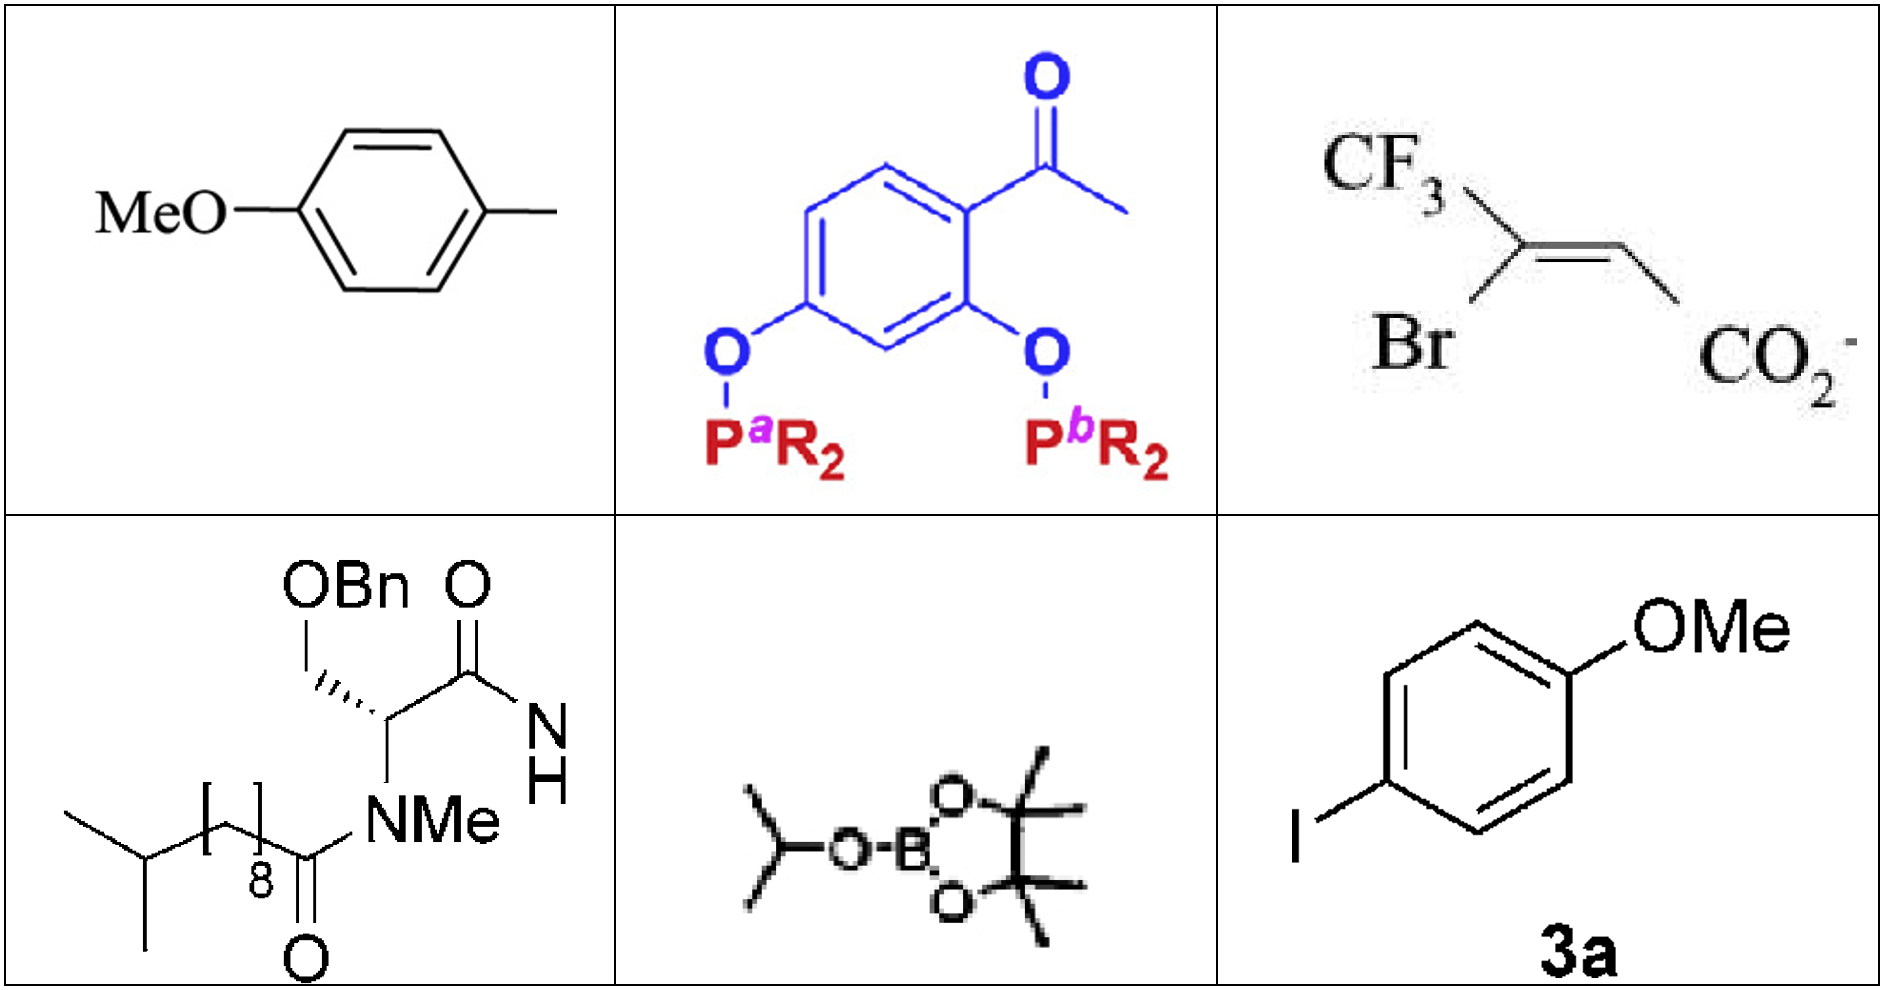
\includegraphics[scale=0.3]{imagenes/positive_examples.png}}  
    \caption{Ejemplos de muestras positivas del \textit{dataset}}
    \label{fig:positive_examples}
\end{figure}

Los ejemplos negativos son, en cambio, imágenes que contienen rectas, curvas y otras figuras que se parecen a las formas que adquiere una molécula, pero no lo son. La diversidad de estas imágenes es muy alta, como se puede observar en la Figura \ref{fig:negative_examples}. En esta categoría hay más imágenes, 800 en total.

\begin{figure}[H]
\centering
    \fbox{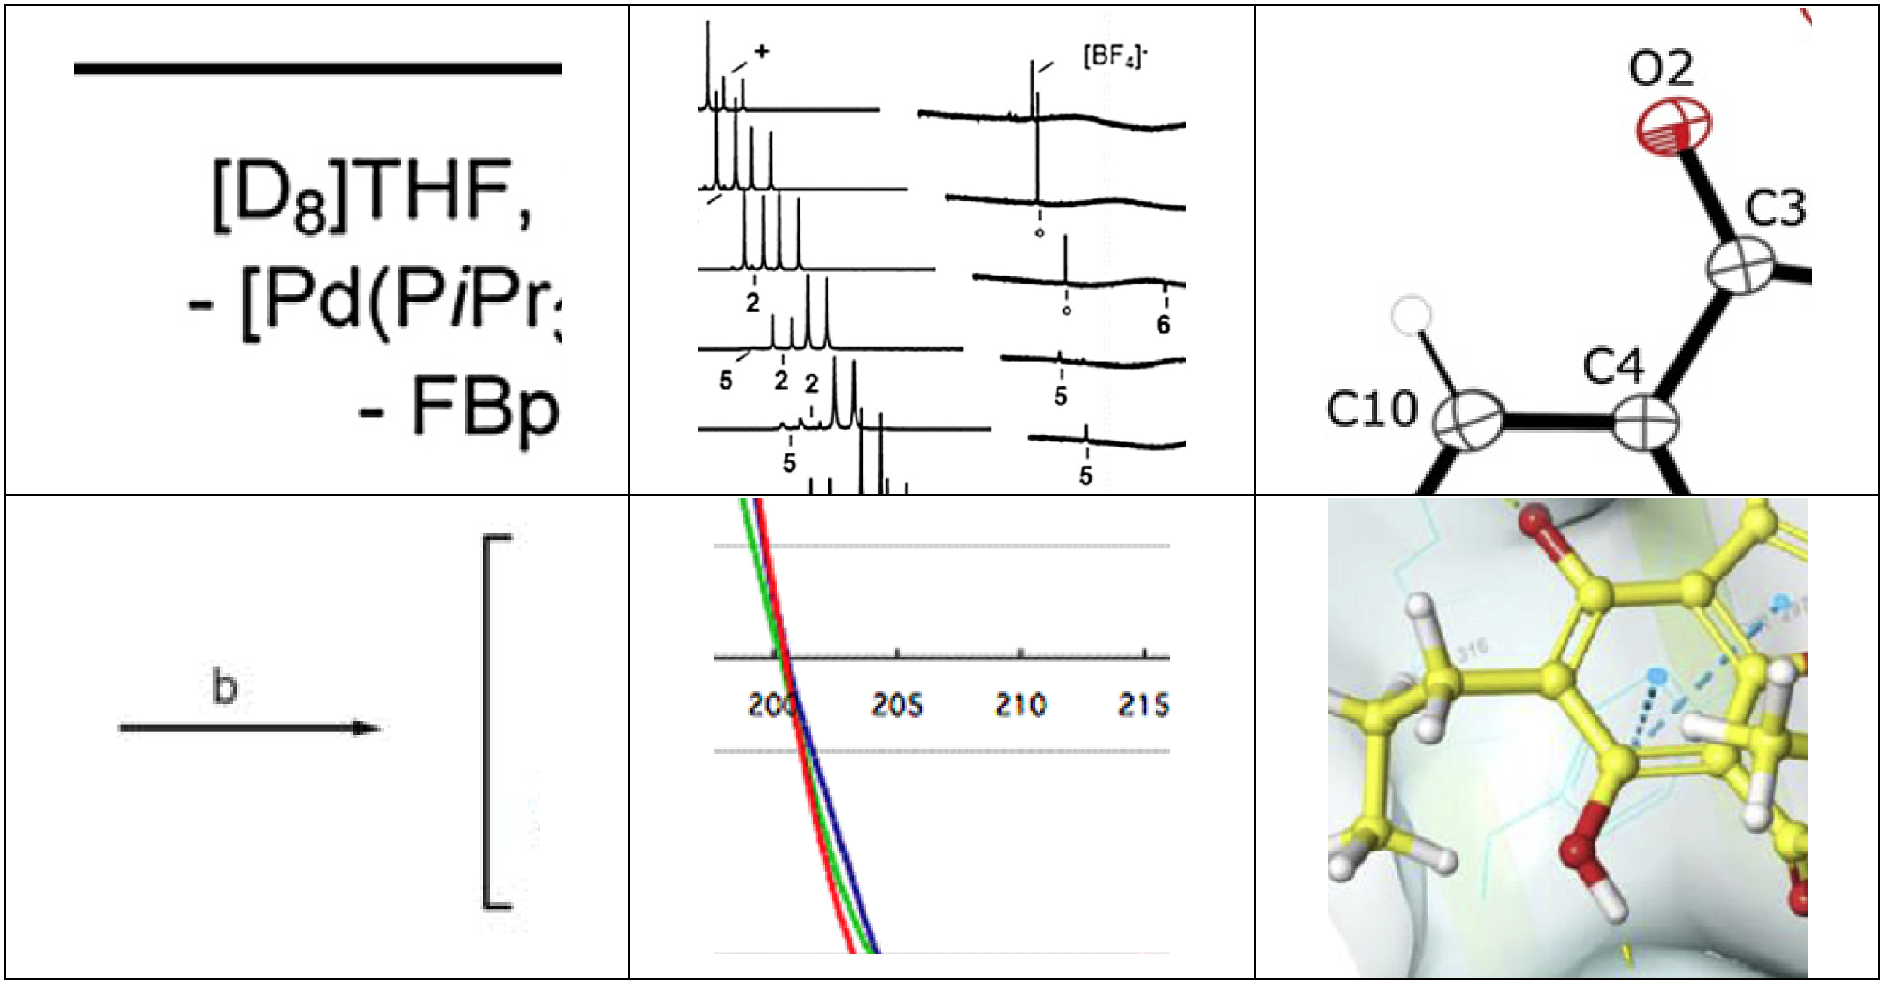
\includegraphics[scale=0.3]{imagenes/negative_examples.png}}  
    \caption{Ejemplos de muestras negativas del \textit{dataset}}
    \label{fig:negative_examples}
\end{figure}

Estas imágenes necesitan un preprocesamiento, es necesario elegir el formato con el que se va a trabajar y dimensionarlas para que todas tengan el mismo tamaño. Debido a que el canal alfa del formato .png no se está aprovechando, decido convertirlas a formato .jpg y así trabajar con tres canales en los modelos. Además, el modelo generativo que se utiliza está diseñado para trabajar con imágenes con este número de canales, así que será lo más adecuado.

Lo más conveniente sería dimensionar todas las imágenes al tamaño de la más grande, así no se perdería información. Pero esto puede suponer un problema, ya que existen algunas que superan los 700x700 píxeles, y cuanto mayor es su resolución más parámetros necesitan almacenar los modelos, dando lugar a altos tiempos de ejecución, y sobre todo, a problemas con la memoria de la GPU. Las GPUs del clúster no tienen capacidad para almacenar modelos con tantos parámetros, por lo que decido reducir el tamaño de las imágenes a 256x256. 

También mencionar el limitado número de ejemplos positivos que existen en comparación con negativos: estamos ante un conjunto de datos desbalanceado. En el momento de entrenar el clasificador, habrá que conseguir que esté más balanceado, ya sea reduciendo el número de ejemplos negativos utilizado o aplicando \textit{data augmentation} sobre los positivos. En este trabajo elijo la segunda opción, ya que en aprendizaje automático cuantos más datos se utilizan en el entrenamiento, mejores modelos se obtienen. 

La técnica de \textit{data augmentation} consiste en aumentar el tamaño del conjunto de datos completándolo con imágenes alteradas de este. Existen bibliotecas en lenguajes de programación como Python que facilitan en gran medida esta tarea, ya que permiten indicar, entre una serie de transformaciones ya implementadas, cuáles queremos aplicar \cite{imgaug}. En este caso se van a crear tres \textit{data augmentation} diferentes, y comprobaremos cuál funciona mejor en los experimentos. La primera realizará transformaciones suaves, la segunda algo más fuertes y la tercera bastante disruptivas.

\noindent\rule{\textwidth}{1pt}
\noindent\textit{Data augmentation} 1. Transformaciones suaves:
\vspace{-0.2cm}
\\\noindent\rule{\textwidth}{1pt}
\begin{itemize}
    \item A\_veces(50\%, DesenfoqueGaussiano(sigma=[0, 0.5]))
    \item Escalar(x: [80\%, 100\%], y: [80\%, 100\%])
    \item Rotar([-25º, +25º])
    \item Estirar([-5,5])
\end{itemize}
\vspace{-0.3cm}
\noindent\rule{\textwidth}{1pt}


A cada imagen del conjunto de datos se le aplicarán estas cuatro transformaciones, la primera solamente con un 50\% de probabilidad. Los parámetros de cada transformación vienen dados en un rango, de forma que se elige un valor aleatorio en este.

\noindent\rule{\textwidth}{1pt}
\noindent\textit{Data augmentation} 2: Transformaciones más fuertes
\vspace{-0.2cm}
\\\noindent\rule{\textwidth}{1pt}
\begin{itemize}
    \item A\_veces(50\%, DesenfoqueGaussiano(sigma=[0, 0.5]))
    \item ContrasteLineal([0.75, 1.5])
    \item Escalar(x: [70\%, 100\%], y: [70\%, 100\%])
    \item Rotar([-45º, +45º])
    \item Estirar([-10,10])
    \item Trasladar(x: [-10\%, 10\%], y: [-10\%, 10\%])
    \item Multiplicar([0.8, 1.2], por\_canal=25\%)
    \item RuidoGaussianoAditivo(loc=0, escala=[0.0, 0.05*255])
    \item VoltearIzdaDcha(30\%)
\end{itemize}
\vspace{-0.3cm}
\noindent\rule{\textwidth}{1pt}


En este caso, utilizo transformaciones como Multiplicar (multiplica el valor de los píxeles de la imagen por un número entre 0.8 y 1.2), RuidoGaussianoAditivo (donde a cada píxel se le añade ruido generado mediante una distribución gaussiana centrada en 0 y con desviación entre 0 y 0.05*255) o VoltearIzqdaDcha, entre otras.

\noindent\rule{\textwidth}{1pt}
\noindent\textit{Data augmentation} 3: Transformaciones fuertes
\vspace{-0.2cm}
\\\noindent\rule{\textwidth}{1pt}
\begin{itemize}
    \item A\_veces(50\%, DesenfoqueGaussiano(sigma=[0, 0.6]))
    \item ContrasteLineal([0.75, 2])
    \item Escalar(x: [70\%, 100\%], y: [70\%, 100\%])
    \item Rotar([-45º, +45º])
    \item Estirar([-10,10])
    \item Trasladar(x: [-20\%, 20\%], y: [-10\%, 10\%])
    \item Multiplicar([0.6, 1.4], por\_canal=25\%)
    \item RuidoGaussianoAditivo(loc=0, escala=[0.0, 0.05*255], por\_canal=30\%)
    \item VoltearIzdaDcha(20\%)
    \item VoldearArribaAbajo(20\%)
    \item A\_veces(70\%, TransformacionElastica(alfa=[0.75, 3], sigma=(0.2, 0.5)))
    \item UnoEntre(Nitidez(alfa=[0, 1], brillo=[0.5, 1.5]), Repujar(alfa=[0, 1], fuerza=[0.75, 2]))
    \item Dropout([0.01, 0.15], por\_canal=0.5)
\end{itemize}
\vspace{-0.3cm}
\noindent\rule{\textwidth}{1pt}


Finalmente, en esta versión de \textit{data augmentation} añado transformaciones que alteran en gran medida el aspecto de las imágenes. TransformacionElastica desplaza píxeles de una zona de la imagen a otra cercana, donde alfa controla la distancia con la que se produce el desplazamiento y sigma la suavidad de este, un valor bajo de sigma dará lugar a imágenes ruidosas y pixeladas. Nitidez aplica este efecto a la imagen y mezcla el resultado con la imagen original, la intensidad de la mezcla se controla con el parámetro alfa, mientras que el parámetro brillo controla el brillo de la imagen. Repujar (\textit{Emboss} en inglés) da a la imagen un aspecto metálico, pronunciando las altas luces y sombras. Por último, Dropout da el valor 0 a cada pixel con una probabilidad entre 0.01 y 0.15. 

Todas estas transformaciones se aplican en un orden aleatorio, lo que aporta una mayor diversidad. Como resumen, la Figura \ref{fig:datasets} recoge los diferentes conjuntos de datos que obtendremos tras este proceso de \textit{data augmentation}.
\begin{figure}[H]
\centering
    \fbox{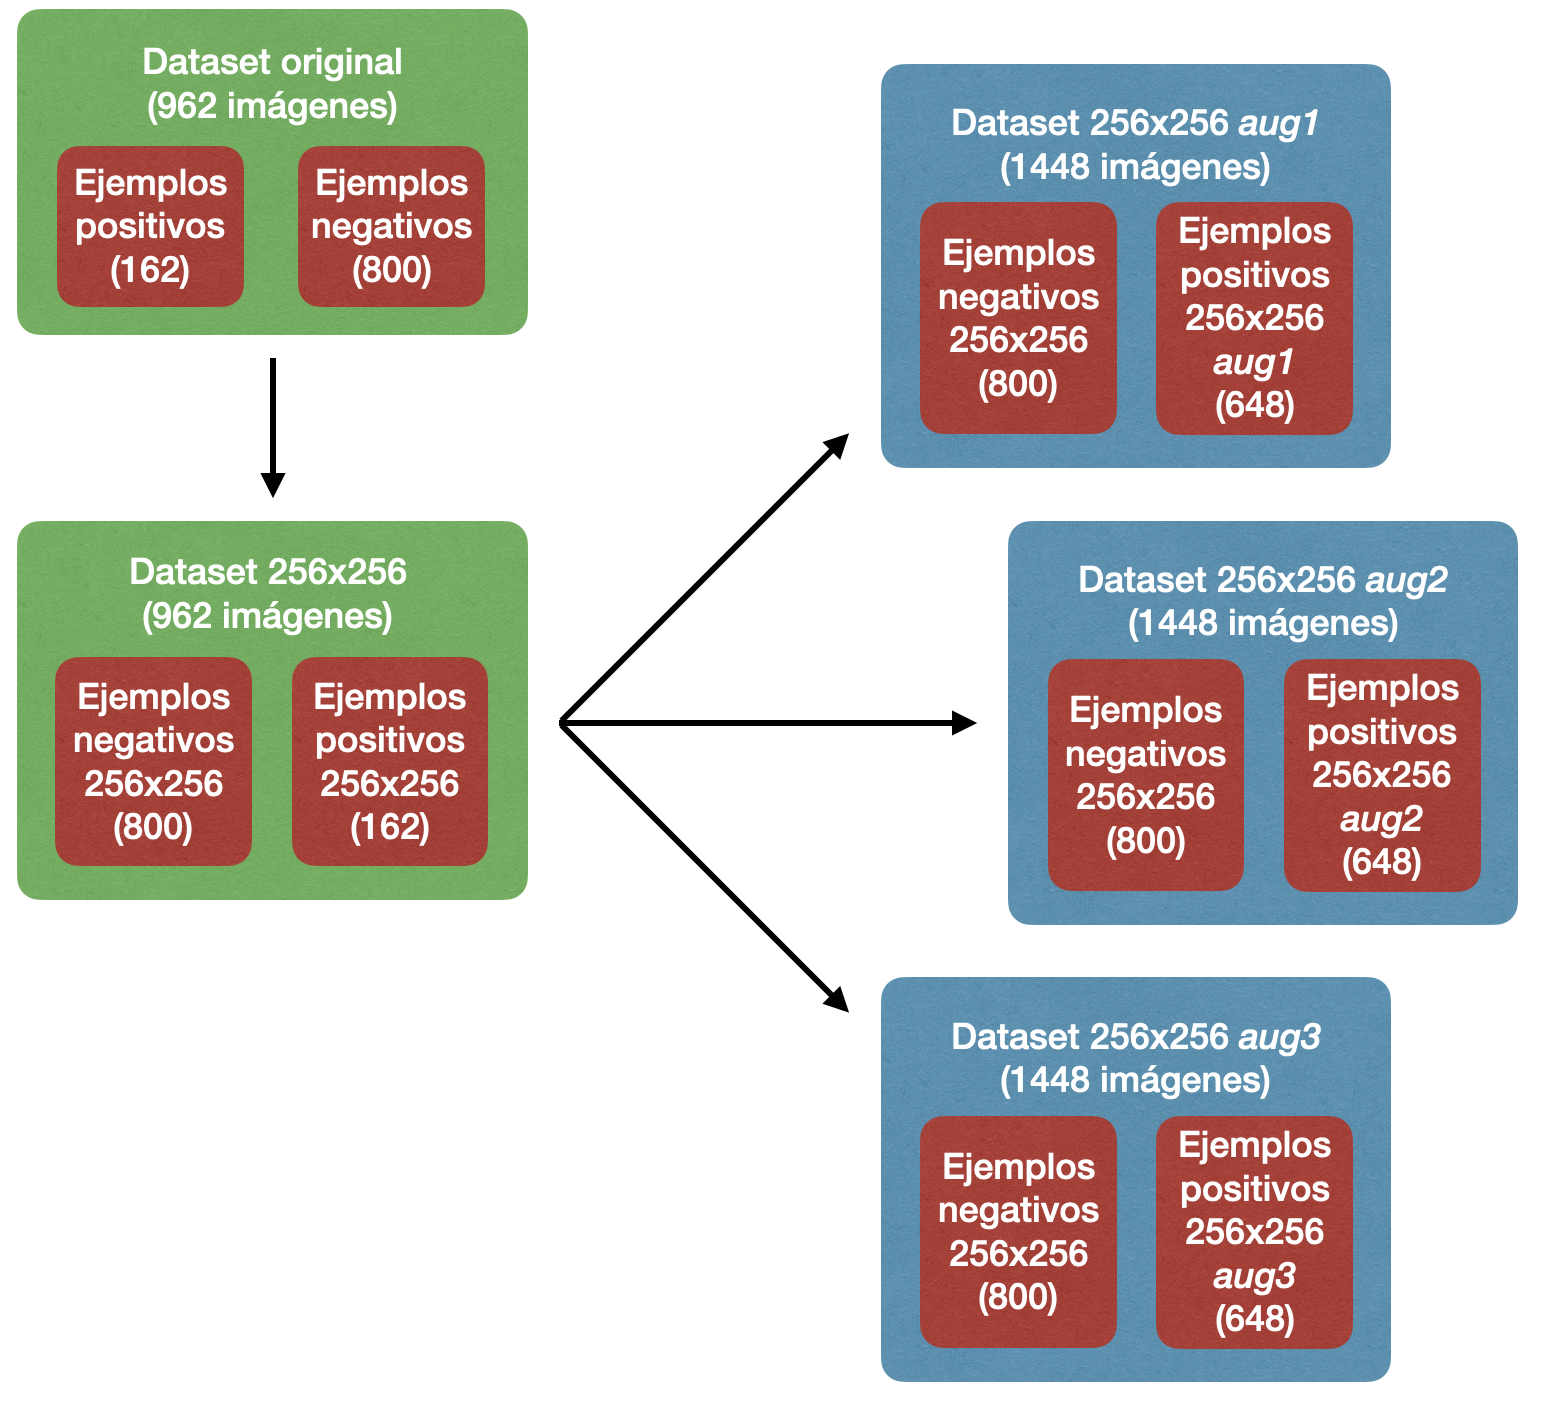
\includegraphics[scale=0.42]{imagenes/metodologia/datasets.png}}  
    \caption{Diferentes \textit{datasets} generados a partir del original}
    \label{fig:datasets}
\end{figure}

Las secuencias \textit{data augmentation} se aplicarán en tres ocasiones sobre el conjunto de ejemplos positivos, por lo que cuadruplican su tamaño inicial: 162 + 3*162 = 648

Ahora ya tengo un \textit{dataset} razonablemente balanceado (800 ejemplos negativos vs 648 positivos), bueno, en concreto tres \textit{datasets}. Tras realizar las pruebas experimentales decidiré cuál es el más adecuado, de forma que las imágenes generadas mediante \textit{data augmentation} aporten una diversidad razonable al conjunto pero sin excederse, para posteriormente utilizarlo para entrenar el clasificador.

\newpage
\section{Generación de \textit{hard negatives}}
Tras balancear los \textit{datasets} con \textit{data augmentation}, se procede a generar \textit{hard negatives}. Este tipo de ejemplos negativos son aquellos que se encuentran en el límite de lo que es negativo y positivo, aquellos que a los modelos de aprendizaje automático les cuesta clasificar. Incorporar este tipo de imágenes al conjunto de entrenamiento permite que el modelo sea más preciso en casos extremos y por tanto que funcione mejor. La Figura \ref{fig:hard-negatives} muestra el concepto de \textit{hard negative} de forma visual.

\begin{figure}[H]
\centering
    \fbox{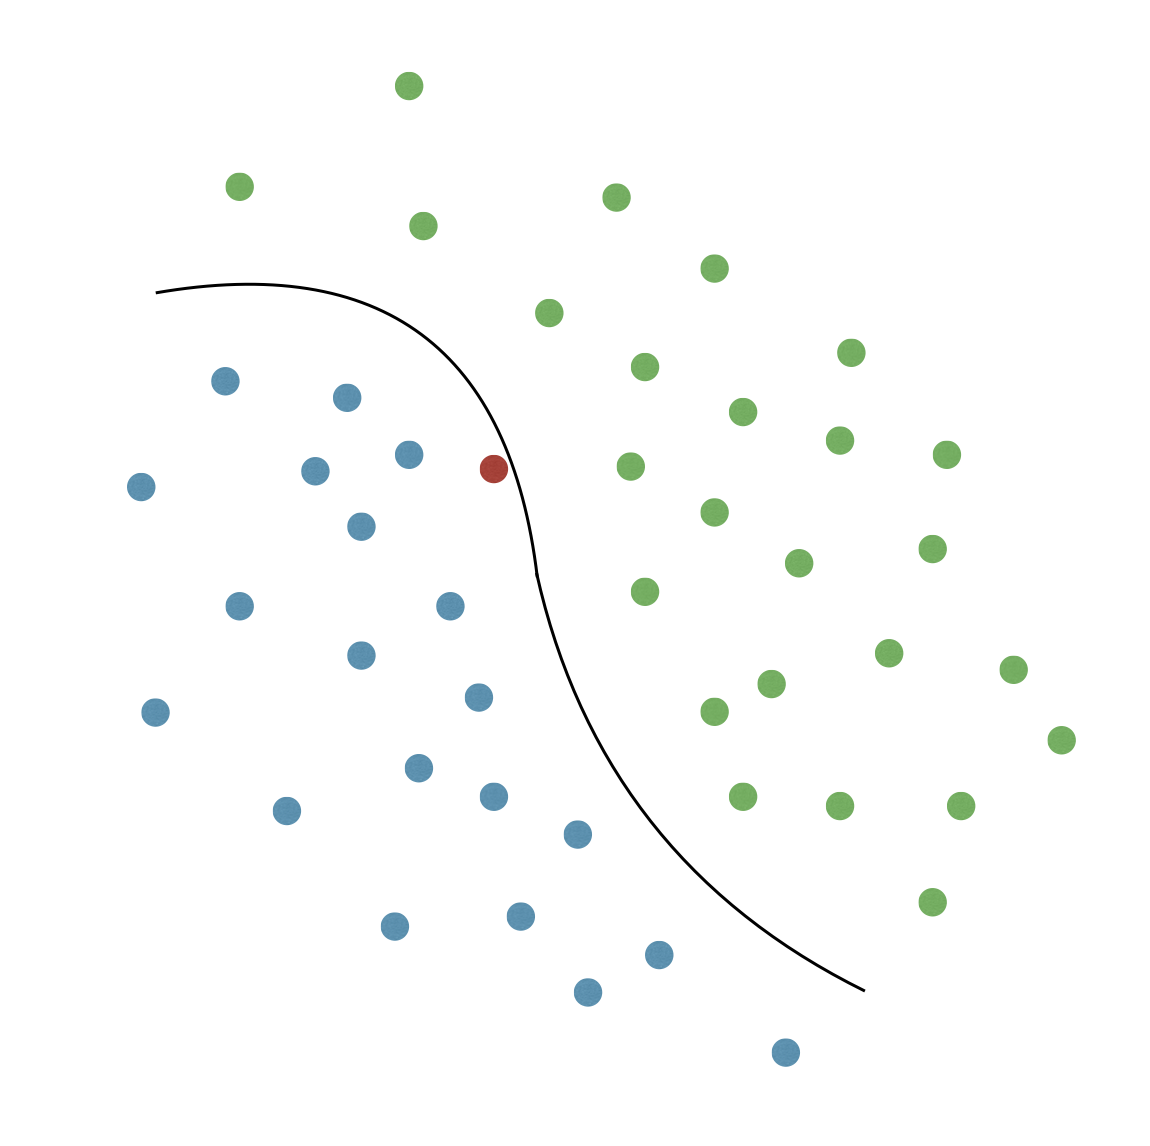
\includegraphics[scale=0.36]{imagenes/metodologia/hard_negatives.png}}  
    \caption{Límite de decisión separando dos clases. El individuo en rojo representa un \textit{hard negative} perteneciente a la clase azul, ya que se encuentra muy cercano al límite de decisión.}
    \label{fig:hard-negatives}
\end{figure}

La generación de estos ejemplos la voy a realizar utilizando el modelo desarrollado por Esser et al. \cite{esser2021taming}, descrito en la Sección \ref{taming-transformers}. Para ello, entrenaré el modelo sobre los ejemplos positivos del conjunto de datos, de forma que sea capaz de generar imágenes que recuerden a moléculas sin que sean demasiado realistas. 

Se entrenará el modelo sobre los tres conjuntos de datos aumentados, aunque también se realizarán pruebas sobre el \textit{dataset} original. El entrenamiento se realizará durante diferentes épocas, y se comprobará visualmente cuál es el número adecuado. En concreto, sobre cada conjunto de datos, se prevé probar con 70, 90, 110, 130, 150 y 170 épocas. Si fuera necesario realizar más experimentos con diferentes valores, se realizarían también. Discutiré esto más a fondo en el capítulo siguiente.

\begin{figure}[H]
\centering
    \fbox{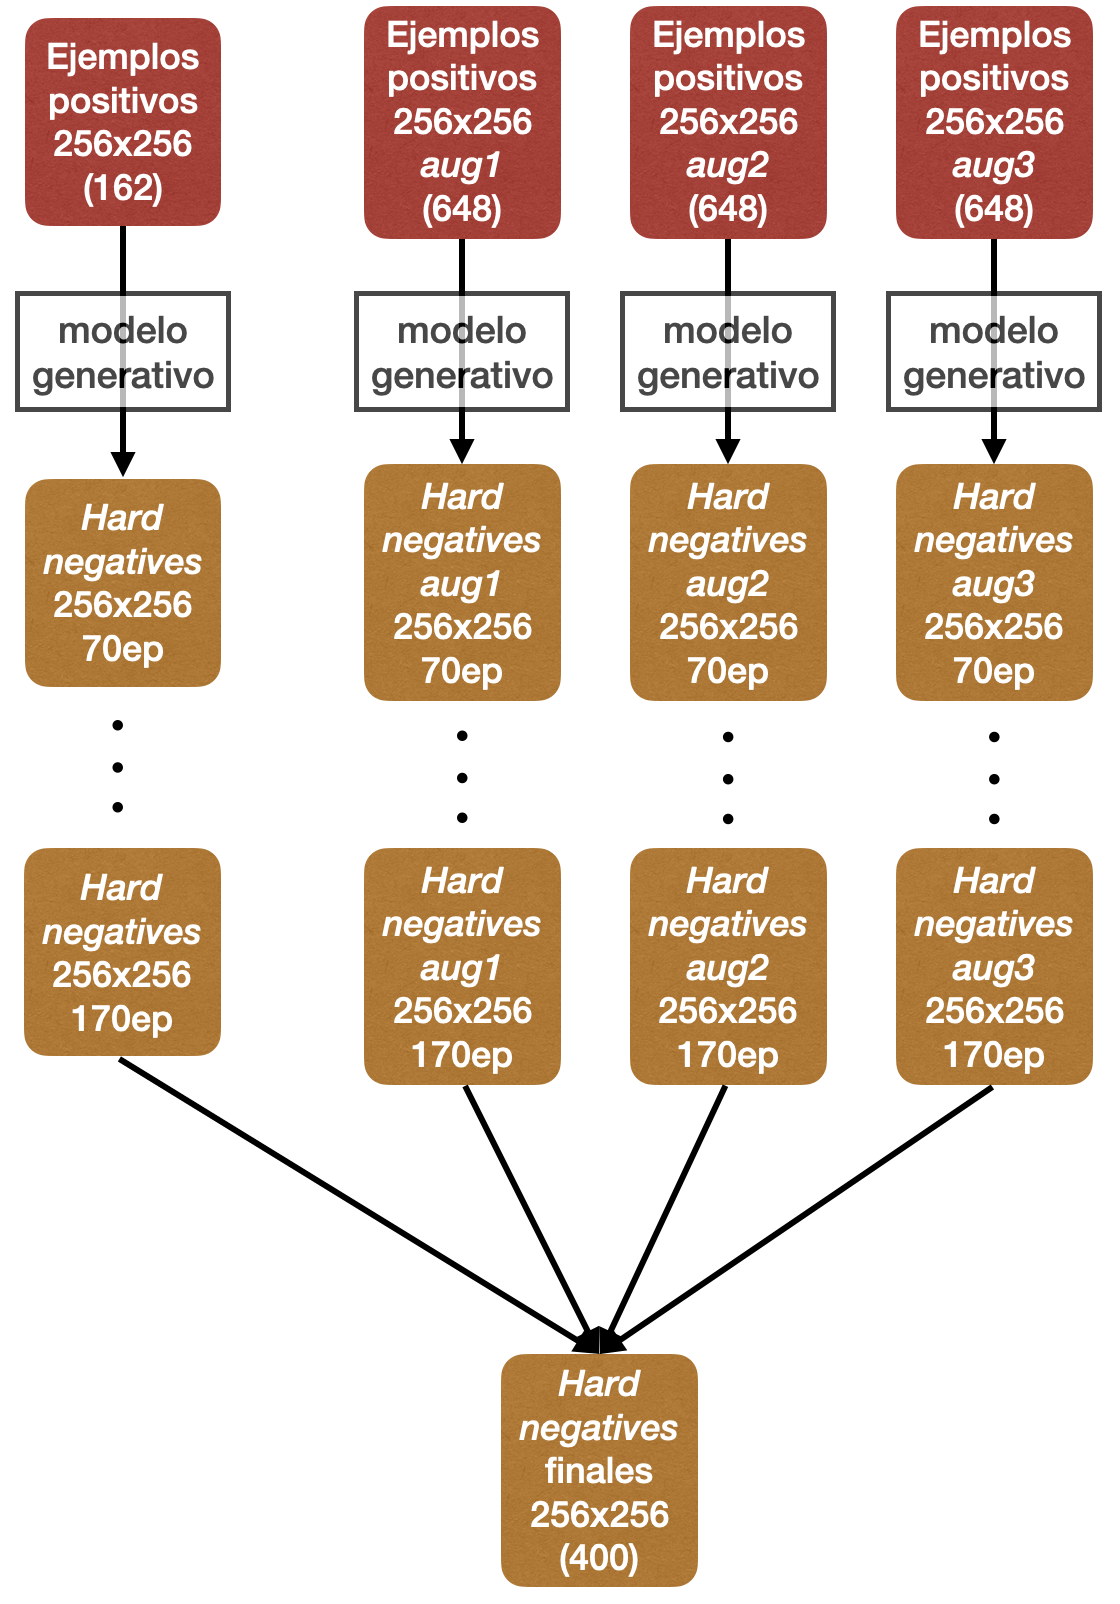
\includegraphics[scale=0.42]{imagenes/metodologia/generate_hard_negatives.png}}  
    \caption{Diferentes \textit{hard negatives} obtenidos entrenando el modelo con diferentes \textit{data augmentation} y número de épocas.} 
    \label{fig:generate-hard-negatives}
\end{figure}
    
Tras realizar los experimentos, se escogerá el modelo (o los modelos) que generen \textit{hard negatives} de mayor calidad. Esta elección se realizará de forma visual. Con los modelos elegidos se creará un conjunto de \textit{hard negatives} finales (Figura \ref{fig:generate-hard-negatives}).

\newpage
\section{Clasificación de imágenes}
El segundo objetivo de este proyecto consiste en construir un clasificador capaz de separar las imágenes que contienen estructuras de moléculas de aquellas que no. Hasta ahora se ha preparado el \textit{dataset} con el que se va a entrenar este modelo y se han generado \textit{hard negatives} que pueden ayudar a crear un clasificador más robusto.

En concreto voy a trabajar con dos \textit{datasets}, no solo con uno (Figura \ref{two_final_datasets}): el que ha sido balanceado pero no contiene \textit{hard negatives} y el que sí los contiene, 400 ejemplos negativos originales y 400 ejemplos negativos de los generados de forma sintética. Se entregarán a los científicos de la Universidad de Negev dos clasificadores, cada uno entrenado sobre uno de los dos conjuntos de datos. Para implementarlos utilizo la biblioteca PyTorch, ya expuesta en la Sección \ref{pytorch}.

\begin{figure}[H]
\centering
    \fbox{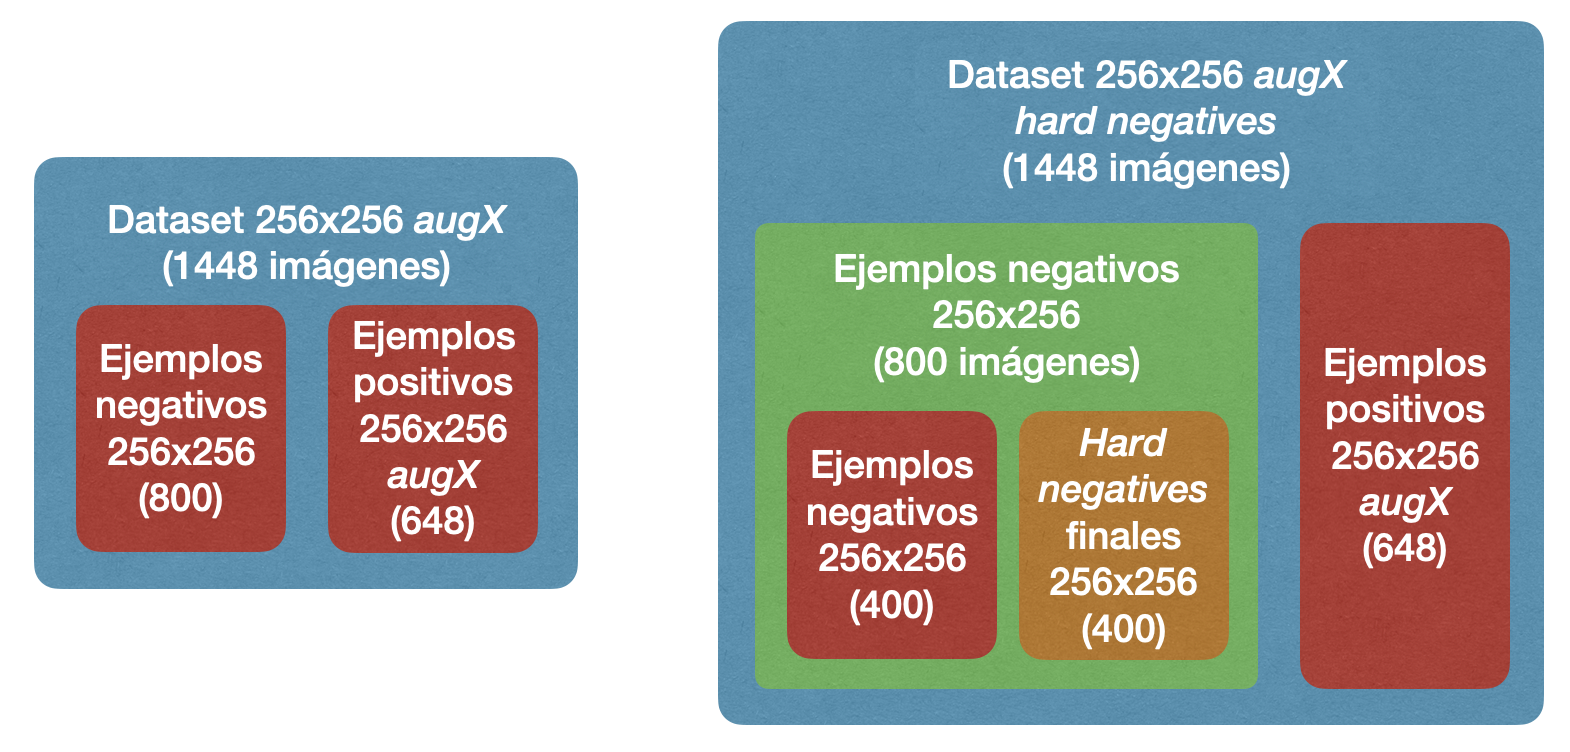
\includegraphics[scale=0.42]{imagenes/metodologia/two_datasets.png}}  
    \caption{Dos \textit{datasets} para entrenar dos clasificadores.} 
    \label{fig:two_final_datasets}
\end{figure}

A priori no se puede conocer que arquitectura funcionará mejor para este problema, por lo que se implementarán varias y se comparará su rendimiento. Voy a elegir una de tamaño pequeño, otra de tamaño mediano y otra de tamaño grande y comparar cuál es la más adecuada:
\begin{itemize}
    \item \textbf{LeNet5:} Modelo propuesto por Yann LeCun en 1998 \cite{lecun1998gradient}, fue una de las primeras redes convolutivas de la historia. Se diseñó con el propósito de reconocer imágenes de dígitos numéricos, y tras compararse su rendimiento con otros modelos en uso, se demostró que los sobrepasaba. Esto atrajo a muchos investigadores a esta incipiente línea de investigación y sentó las bases para las arquitecturas del futuro.
    \item \textbf{AlexNet:} Propuesto por Alex Krizhevsky en 2012 \cite{krizhevsky2012imagenet}, consiguió mejorar por un alto porcentaje a la siguiente mejor solución en el concurso ImageNet Large Scale Visual Recognition Challenge. La ventaja de este modelo frente a otros fue su profundidad, que le permitía reconocer imágenes más complejas con mayor precisión. Esto conllevó un aumento del número de parámetros y del tiempo de entrenamiento, que fue contrarrestado por el uso de GPUs que permitieron la paralelización. Para combatir el sobreajuste se utilizó \textit{dropout}, donde los enlaces entre neuronas se desconectaban con una determinada probabilidad durante cada iteración del entrenamiento.
    \item \textbf{VGG16:} Desarrollado por el Visual Geometry Group (de sus siglas procede el nombre del modelo) de la Universidad de Oxford \cite{https://doi.org/10.48550/arxiv.1409.1556}, fue el ganador del concurso ImageNet en su edición de 2014. Una de las características que le permitió mejorar frente a otros modelos fue el uso de \textit{kernels} convolutivos de pequeño tamaño (3x3). Se presentaron varias versiones del algoritmo, cada una con un número de capas diferente. La que nosotros utilizamos, VGG16, cuenta con 16 capas.
\end{itemize}

En un principio, cada uno de estos modelos se diseñó para trabajar con un tamaño de imágenes y de salida específicos, pero los voy a adaptar para funcionar sobre imágenes 256x256 y vectores \textit{one-hot}. Estos vectores se utilizan en problemas de clasificación, de forma que cada coordenada del vector representa una de las clases (en nuestro caso dos clases, imagen de molécula o no). Cada coordenada se conoce como \textit{logit}.

Tras la implementación con estos cambios, el número de parámetros se incrementa. Por ejemplo, LeNet5 contaba originalmente con 62006 parámetros al trabajar con imágenes 28x28 y un vector de salida de tamaño 10, pero tras los cambios cuenta con 7393806. Las versiones modificadas de AlexNet y VGG16 cuentan respectivamente con 58289538 y 153263298 parámetros.

Cada uno de estos modelos tiene diferentes hiperparámetros configurables: el tamaño del lote de entrenamiento (\textit{batch size}), el optimizador que modifica los parámetros en cada iteración, la inicialización de los pesos, etc. Determinados valores en estos hiperparámetros hacen que los modelos produzcan peores o mejores resultados, por lo que es importante elegir valores adecuados. Es imposible probar todos los valores posibles, por lo que selecciono algunos que creo que pueden dar buenos resultados, realizando una comparativa: esto es lo que se conoce como \textit{grid search}.

Voy a trabajar modificando tres hiperparámetros. Aunque podríamos hacer pruebas con más, el número de modelos a entrenar crecería exponencialmente:
\begin{itemize}
    \item \textbf{Tasa de aprendizaje (\textit{Learning rate}):} Es probablemente el más importante. Si se le da un valor demasiado bajo, los pesos del modelo variarán en muy poca medida en cada iteración y el error decrecerá muy lentamente. Si su valor es muy alto, es posible que el valor de los pesos y del error oscile y el algoritmo no converja. Es conveniente probar con diferentes posibilidades: en este caso se va a comprobar el rendimiento de los modelos tomando 0.5, 0.05, 0.005, 0.0005 y 0.00005 como posibles valores. \cite{berzal2018redes}
    \item \textbf{Inicialización de los pesos:} Las redes neuronales dependen en gran medida de la inicialización de los pesos. Si todas las neuronas se inicializasen con el mismo valor, el modelo no sería capaz de aprender nada, ya que la derivada del gradiente sería la misma para todas. Las que voy a utilizar son: \cite{pytorch-doc}
    \begin{itemize}
        \item \textit{He:} utilizada por defecto en PyTorch en sus capas completamente conectadas y convolutivas, He (también conocida como Kaiming) genera valores aleatorios a partir de una distribución uniforme $\mathcal{U}(-bound, bound)$, donde $bound = gain * \sqrt{\frac{3}{fan\_in}}$. El parámetro $fan\_in$ depende de la entrada a la neurona. Por otro lado, en la inicialización por defecto de PyTorch $gain$ depende de $a = \sqrt{5}$.
        \item \textit{Xavier:} Los valores aleatorios son generados a partir de una distribución uniforme $\mathcal{U}(-a, a)$, donde $a = \sqrt{\frac{6}{fan\_in + fan\_out}}$. Los parámetros $fan\_in$ y $fan\_out$ dependen de la entrada y de la salida de la neurona respectivamente.
    \end{itemize}
    Una correcta inicialización de los pesos evita el problema de la evanescencia del gradiente (durante el entrenamiento, este se vuelve cada vez menor aproximándose a cero, de forma que los pesos no cambian) y el de la explosión del gradiente (este toma valores cada vez mayores, de forma que los pesos cambian en gran medida y el algoritmo diverge).
    \item \textbf{Algoritmo de optimización:} Como muchos otros algoritmos de aprendizaje automático, los de aprendizaje profundo son problemas de optimización donde se intenta reducir el error de una función objetivo $f$ definida sobre un conjunto de datos de entrenamiento. En muchas ocasiones, este proceso de optimización se realiza de forma numérica, una forma de hacerlo es a partir del cálculo del gradiente descendiente, un proceso costoso por tener que calcular en numerosas ocasiones el valor de la función $f$ y de su derivada. La elección del algoritmo de optimización es importante, ya que de él dependen la convergencia a una buena solución y el actualizar los pesos de forma eficiente: \cite{berzal2018redes}
    \begin{itemize}
        \item \textit{SGD:} En el entrenamiento de redes neuronales, el gradiente se calcula a partir de los datos de entrenamiento. Si estos datos no son un conjunto representativo de la distribución real porque contienen ruido, la estimación no será correcta. El gradiente se puede calcular a partir de todos los datos de entrenamiento (aprendizaje por lotes), a partir de un subconjunto (aprendizaje por minilotes) o a partir de una única muestra (aprendizaje online). Cuantos más datos se utilicen para calcular el gradiente, menor será el error cometido al estimarlo, pero como se ha mencionado, los datos siempre pueden contener ruido y por tanto no se puede asegurar que los resultados sean correctos. El gradiente descendiente estocástico (\textit{Stochastic Gradient Descent}, SGD) engloba el aprendizaje por minilotes y el online, y aunque pueda parecer lo contrario por utilizar menos muestras en el cómputo del gradiente, mejora los resultados al permitir al algoritmo escapar de puntos de silla. Además, es mucho más eficiente ya que solo tiene en cuenta un número limitado de datos en el cómputo.
        \item \textit{AdaDelta:} Es una extensión de AdaGrad (\textit{Adaptative Gradients}), un optimizador que dota a cada parámetro de una tasa de aprendizaje independiente y que va actualizando su valor durante la ejecución del algoritmo. AdaDelta resuelve el principal problema de Adagrad, la disminución prematura de las tasas de aprendizaje. Esto se debe a que Adagrad las calcula a partir del gradiente acumulado de todas las iteraciones, en cambio AdaDelta sólo utiliza las $n$ iteraciones anteriores.
        \item \textit{Adam:} Se podría considerar una extensión de AdaDelta en la que se utilizan momentos. En concreto, este algoritmo calcula la estimación del primer momento del gradiente (media) y del segundo momento (varianza). A partir de ellos se define la fórmula que da nombre a este algoritmo.
    \end{itemize}
\end{itemize}

En las ejecuciones que voy a realizar, la función de coste utilizada es la función de entropía cruzada (\textit{Cross Entropy Loss}). Esta función integra la función de activación \textit{Softmax}, de forma que cada logit es transformado en un valor probabilístico entre 0 y 1. 

El algoritmo de aprendizaje intentará minimizar el valor de la función de entropía cruzada, es decir, tratará de minimizar la distancia entre las probabilidades devueltas por el modelo y la probabilidad real. Tras el entrenamiento, cuando se realice una predicción, la clase a la que pertenecerá la muestra será aquella que esté representada por el \textit{logit} con mayor probabilidad (Ver Figura \ref{fig:cross-entropy-loss}). \cite{crossentropyloss}


\begin{figure}[H]
\centering
    \fbox{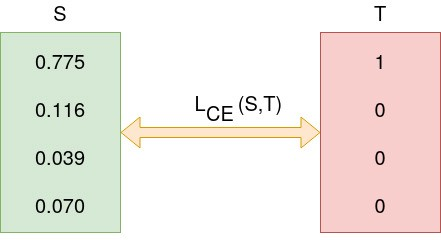
\includegraphics[scale=0.55]{imagenes/image_classification/crossentropyloss.jpeg}}
    \caption{La función de entropía cruzada $L_{CE}$ mide la distancia entre la probabilidad representada en el \textit{logit} $S$ y la probabilidad real representada mediante $T$ \cite{crossentropyloss}. Durante el entrenamiento, el algoritmo tratará de minimizar esta distancia.}
    \label{fig:cross-entropy-loss}
\end{figure}

Hay otro hiperparámetro que fijo desde el inicio que es el tamaño de los minilotes. Podría haber probado con tamaños diferentes, pero de hacerlo la complejidad de la \textit{grid search} crecía en gran medida. Un valor adecuado es aquel que permita que el minilote quepa en la caché de la GPU, de forma que se agilicen los cálculos. Valores como 32, 64 o 128 suelen ser utilizados en la literatura, así que elijo fijar 32. \cite{batch-size}

El objetivo es realizar la \textit{grid search} sobre los dos \textit{datasets} que he comentado, de esta forma compararemos el rendimiento de los modelos según los hiperparámetros utilizados y nos quedaremos con aquellos que dan mejores resultados. Estos serán los que utilicen los modelos que entregue a los científicos.

Los \textit{datasets} se dividirán en dos secciones, \textit{train} y \textit{test}. \textit{train} se utilizará para entrenar los modelos finales (y por tanto será la mayor división, 85\%) y test para evaluar su rendimiento final (15\%). Pero en la \textit{grid search} utilizaremos solamente la división de \textit{train}, a la que aplicaremos validación cruzada. Esta técnica pretende estimar el error de forma más fiable repitiendo el proceso de entrenamiento con diferentes subconjuntos. En concreto, se divide aleatoriamente el conjunto en $k$ partes (en nuestro caso $k=5$). En cada iteración ($k$ en total), se utiliza un subconjunto como \textit{test} y el resto como \textit{train}. Este proceso se resume visualmente en la Figura \ref{fig:train-test}. \cite{berzal2018redes}

Finalmente, tras la \textit{grid search} y cuando se haya decidido cuál es la configuración final, se entrenará el modelo final sobre la partición \textit{train} y se dará un valor de error sobre la \textit{test} (Ver Figura \ref{fig:grid-search}). Como ya hemos comentado realmente tendremos dos modelos finales, uno entrenado sobre el \textit{dataset} sin \textit{hard negatives} y otro sobre el que si los tiene.

\begin{figure}[H]
\centering
    \fbox{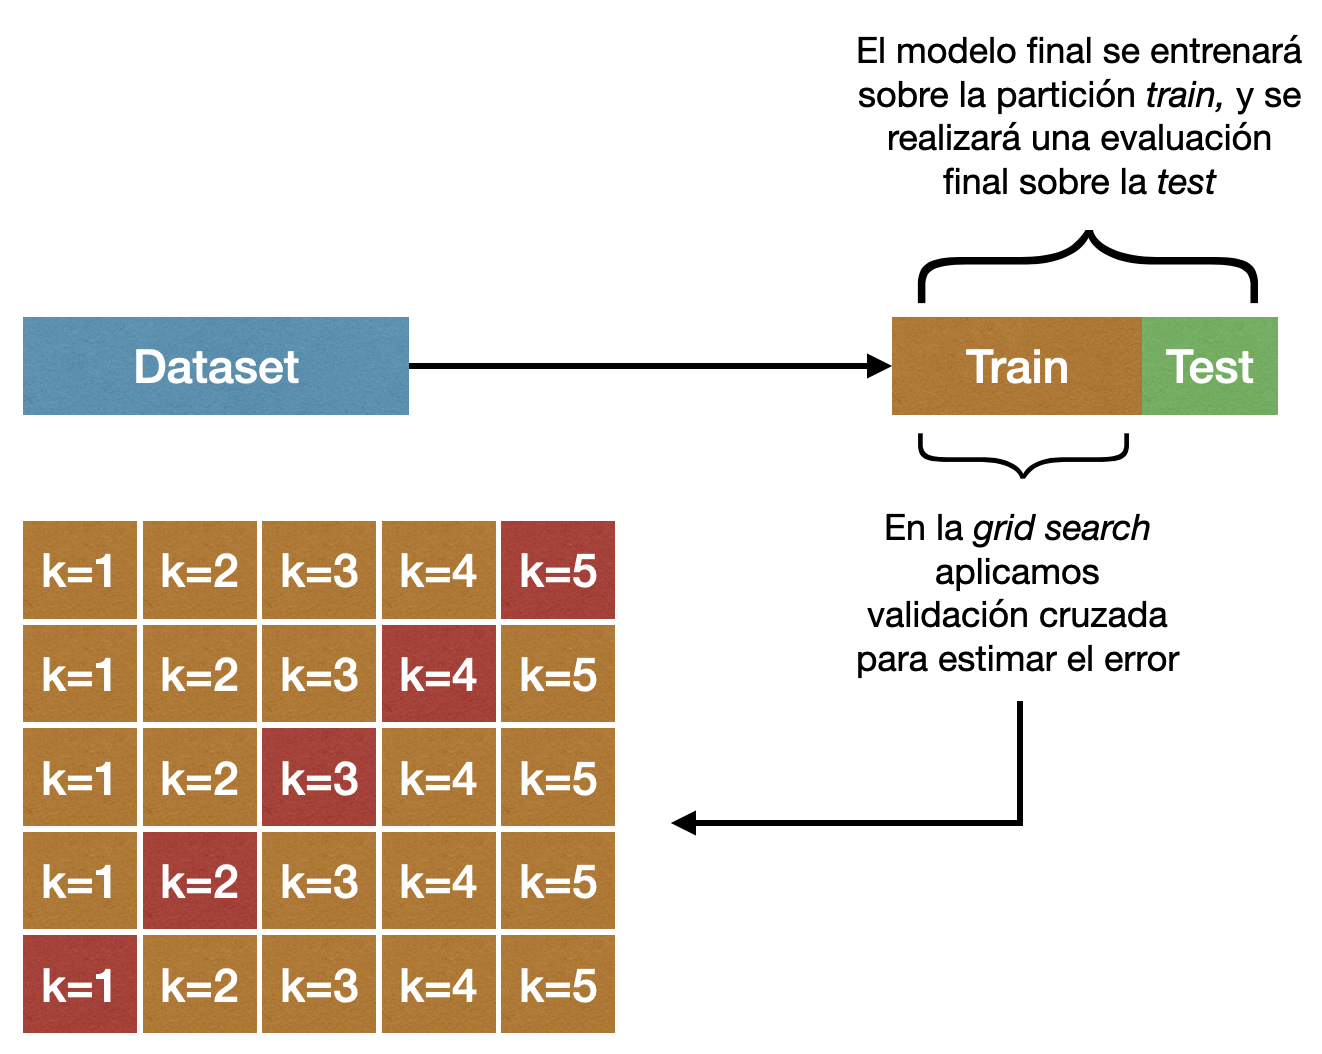
\includegraphics[scale=0.38]{imagenes/metodologia/train_test.png}}  
    \caption{División \textit{train-test}.} 
    \label{fig:train-test}
\end{figure}

\begin{figure}[H]
\centering
    \fbox{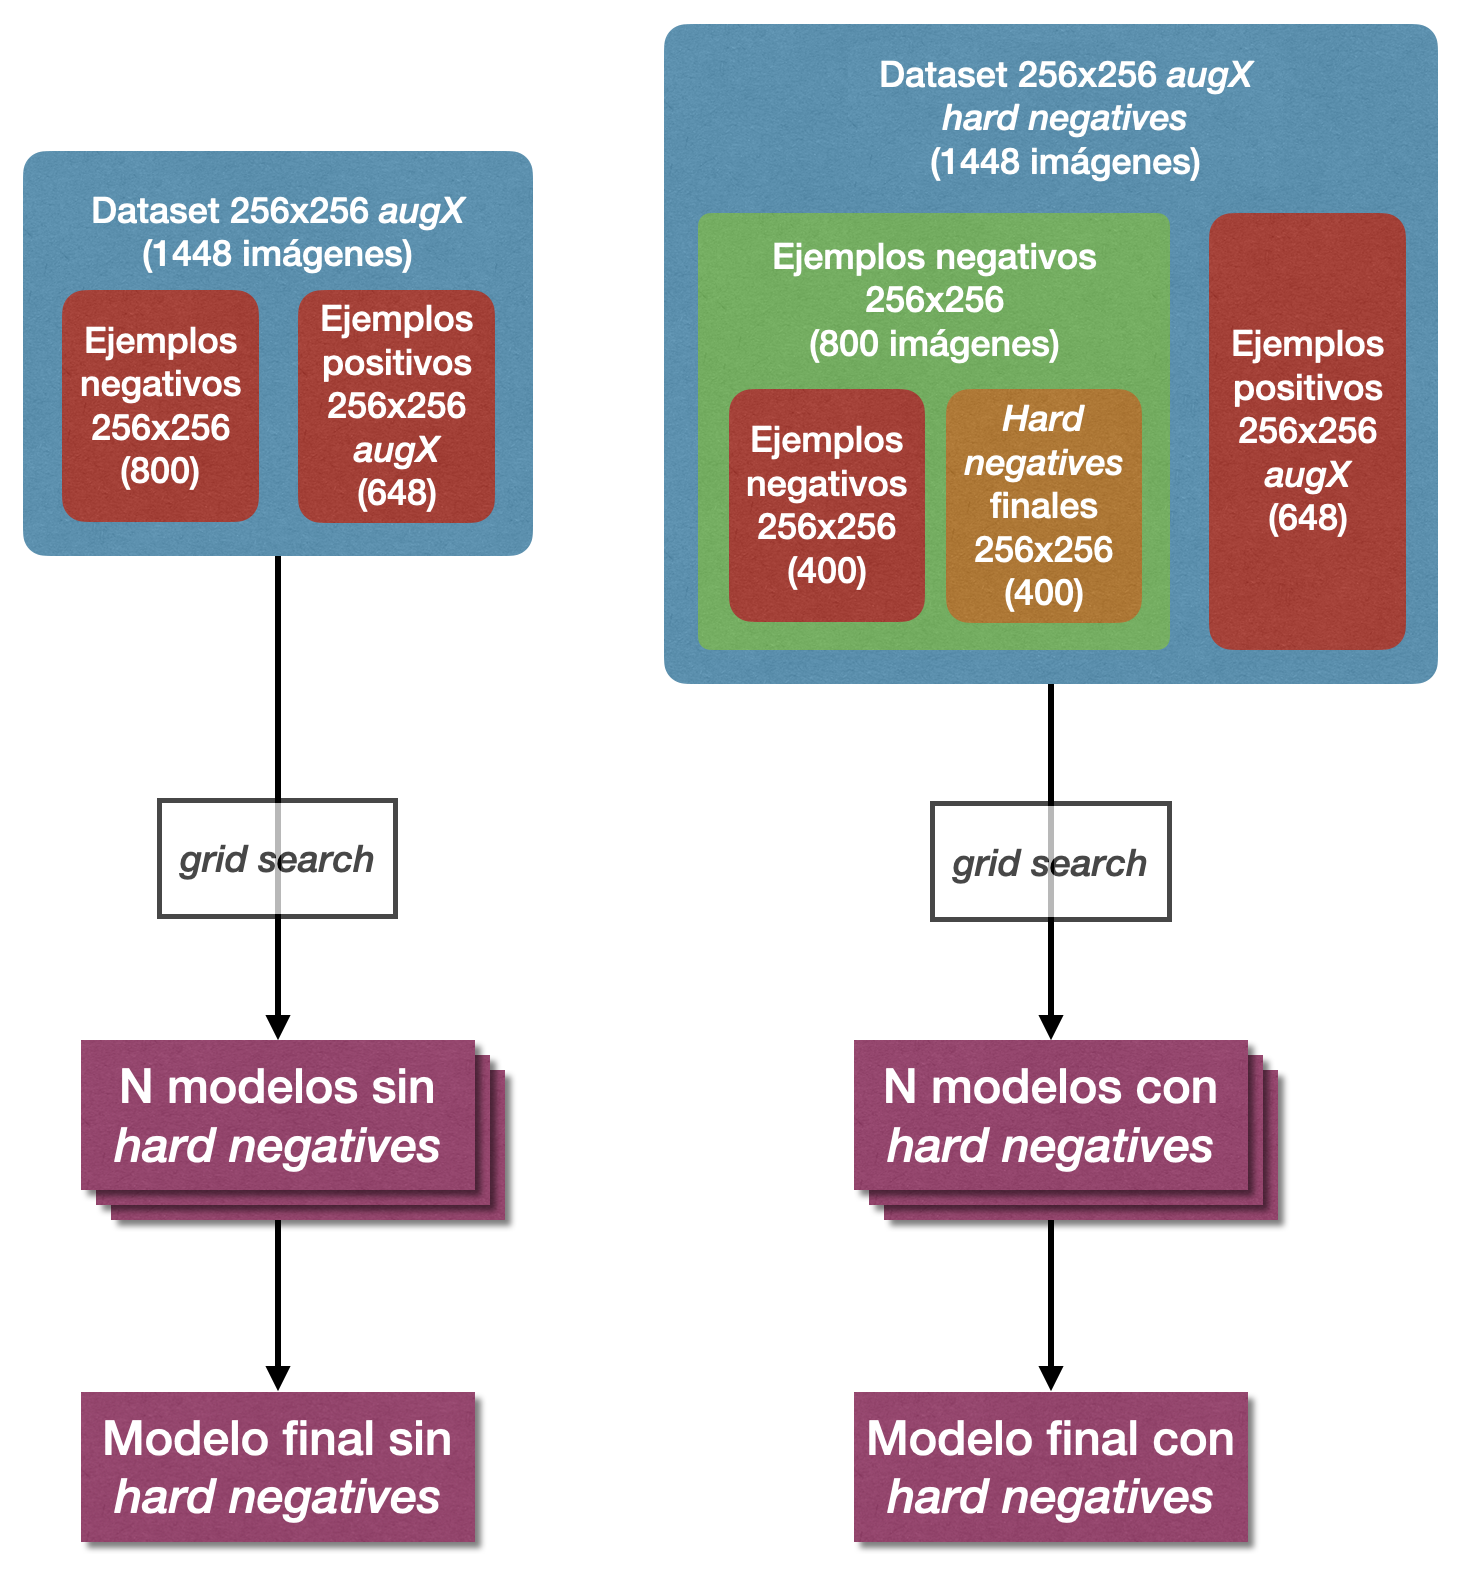
\includegraphics[scale=0.37]{imagenes/metodologia/grid_search.png}}  
    \caption{Realizo una \textit{grid search} sobre ambos \textit{datasets}, y elijo el modelo que mejor resultado da sobre cada uno de ellos.} 
    \label{fig:grid-search}
\end{figure}